\chapter{Cơ sở lý thuyết}
\label{ch:theory}

Chương này trình bày các nền tảng lý thuyết làm tiền đề cho việc xây dựng hệ thống đánh giá ESG-washing. Nội dung bao gồm: khung khái niệm ESG và ESG-washing (Mục~\ref{sec:esg_framework}), các khung ngôn ngữ học nền tảng phục vụ xây dựng quy tắc ký hiệu (Mục~\ref{sec:linguistic_frameworks}), các mô hình NLP và kiến trúc Transformer (Mục~\ref{sec:nlp_transformer}), suy luận ngôn ngữ tự nhiên (Mục~\ref{sec:nli}), Neuro-Symbolic (Mục~\ref{sec:neuro_symbolic}), chắt lọc tri thức (Mục~\ref{sec:knowledge_distillation}), và tổng quan các nghiên cứu liên quan (Mục~\ref{sec:related_works}).

\section{ESG và ESG-washing}
\label{sec:esg_framework}

ESG là bộ ba tiêu chí đánh giá tính bền vững và trách nhiệm xã hội của doanh nghiệp, bao gồm ba trụ cột~\cite{buchetti2025literature}:

\begin{itemize}
    \item \textbf{Môi trường (E --- Environmental):} Đánh giá cách doanh nghiệp quản lý các tác động sinh thái, bao gồm phát thải khí nhà kính, tiêu thụ năng lượng, quản lý nước và chất thải, bảo tồn đa dạng sinh học, và các sáng kiến tài chính xanh.
    \item \textbf{Xã hội (S --- Social):} Đánh giá mối quan hệ của doanh nghiệp với các bên liên quan --- nhân viên, khách hàng, cộng đồng --- thông qua các chỉ số về an toàn lao động, bình đẳng giới, phát triển nhân sự, bảo mật thông tin và trách nhiệm cộng đồng.
    \item \textbf{Quản trị (G --- Governance):} Đề cập đến cơ cấu quản lý, đạo đức kinh doanh, chống tham nhũng, quản trị rủi ro và cơ chế giám sát nội bộ.
\end{itemize}

Báo cáo phát triển bền vững là tài liệu công bố định kỳ của doanh nghiệp về các hoạt động ESG, thường tuân theo các chuẩn mực quốc tế như GRI~\cite{gri2021gri} hoặc được lồng ghép trong báo cáo thường niên. Trong bối cảnh toàn cầu, công bố ESG đã chuyển từ hoạt động tự nguyện sang thành phần bắt buộc trong khung báo cáo doanh nghiệp, đặc biệt tại các khu vực pháp lý như Liên minh Châu Âu~\cite{lagasio2024esg}. Tại Việt Nam, các ngân hàng thương mại ngày càng mở rộng phần công bố ESG trong báo cáo thường niên, phản ánh xu hướng hội nhập với thông lệ quốc tế.

ESG-washing là hiện tượng doanh nghiệp tạo ra hình ảnh ESG tích cực giả tạo thông qua các tuyên bố thiếu cơ sở, phóng đại, hoặc chọn lọc có chủ đích~\cite{delmas2011drivers, lyon2015means}. Khái niệm này mở rộng từ ``greenwashing'' truyền thống (chỉ tập trung vào khía cạnh môi trường) sang toàn bộ ba trụ cột ESG.

Delmas và Burbano~\cite{delmas2011drivers} đã xây dựng khung phân tích toàn diện về các yếu tố thúc đẩy greenwashing, phân loại các cơ chế ESG-washing thành ba dạng chính:

\begin{enumerate}
    \item \textit{Công bố chọn lọc (Selective disclosure):} Doanh nghiệp chỉ công bố các chỉ số tích cực, che giấu hoặc bỏ qua các thông tin tiêu cực. Marquis và cộng sự~\cite{marquis2016scrutiny} chứng minh rằng cơ chế này phổ biến hơn trong các môi trường có mức độ giám sát thấp — một đặc điểm phổ biến của các thị trường mới nổi.
    \item \textit{Tuyên bố mơ hồ (Vague claims):} Sử dụng ngôn ngữ không cụ thể, thiếu định lượng --- ví dụ ``cam kết phát triển bền vững'' mà không kèm chỉ tiêu đo lường. Theo lý thuyết tính chính danh (legitimacy theory) của Cho và Patten~\cite{cho2007role}, các tuyên bố này nhằm duy trì tính chính danh của doanh nghiệp trước áp lực xã hội, hơn là phản ánh hành động thực tế.
    \item \textit{Tuyên bố sai lệch (False claims):} Đưa ra thông tin không chính xác hoặc không thể kiểm chứng về hiệu quả ESG.
\end{enumerate}

Lyon và Montgomery~\cite{lyon2015means} bổ sung một cơ chế quan trọng thứ tư: \textit{tuyên bố không được chứng thực} --- các phát biểu tích cực mà không đi kèm bằng chứng hỗ trợ. Đây là dạng ESG-washing phổ biến nhất nhưng cũng khó phát hiện nhất, vì bản thân nội dung phát biểu không chứa thông tin sai sự thật trực tiếp. Nghiên cứu này tập trung vào chính cơ chế này --- đánh giá mức độ mà các tuyên bố ESG được hỗ trợ bởi bằng chứng cụ thể, có thể kiểm chứng trong cùng tài liệu.

Trong lĩnh vực ngân hàng, ESG-washing mang đặc thù riêng do vai trò trung gian tài chính và quản lý rủi ro hệ thống~\cite{lagasio2024esg}. Ngân hàng không chỉ chịu trách nhiệm về hoạt động ESG trực tiếp (tiêu thụ năng lượng, chính sách nhân sự, quản trị nội bộ) mà còn về tác động ESG gián tiếp thông qua danh mục cho vay và đầu tư --- ví dụ, tín dụng xanh, trái phiếu bền vững, hoặc tài trợ dự án có rủi ro môi trường.

Khi thông tin ESG ngân hàng bị thổi phồng, hệ quả có thể lan rộng ra toàn hệ thống tài chính, tương tự các vụ bê bối tại các quỹ đầu tư bền vững trong những năm gần đây~\cite{lipenkova2023detecting}. Ghitti và cộng sự~\cite{ghitti2024agency} chỉ ra rằng vấn đề đại diện trong ESG-washing đặc biệt nghiêm trọng khi thiếu cơ chế giám sát độc lập --- một thực trạng phổ biến tại các thị trường mới nổi.

Tại Việt Nam, mặc dù các ngân hàng ngày càng đẩy mạnh công bố ESG, mức độ cụ thể và khả năng kiểm chứng của các phát biểu vẫn không đồng đều~\cite{buchetti2025literature}, đặt ra nhu cầu cấp thiết về công cụ phân tích tự động, khách quan --- đây chính là động lực thực tiễn của nghiên cứu này.


\section{Khung ngôn ngữ học nền tảng}
\label{sec:linguistic_frameworks}

Để lượng hóa rủi ro ESG-washing ở mức câu, nghiên cứu này vận dụng ba khung lý thuyết ngôn ngữ học làm nền tảng xây dựng hệ thống quy tắc ký hiệu. Các quy tắc này đóng vai vừa hướng dẫn quá trình dán nhãn dữ liệu, vừa được tích hợp trực tiếp vào huấn luyện mô hình thông qua hàm mất mát ngữ nghĩa (Mục~\ref{subsec:semantic_loss}). Bảng tham chiếu đầy đủ các quy tắc và từ khóa được trình bày tại Phụ lục~\ref{appendix:grounded_rules}.


\subsection{Bloom's Taxonomy --- Thang phân loại mục tiêu nhận thức}
\label{subsec:bloom}

Thang phân loại Bloom được phát triển bởi Anderson và Krathwohl~\cite{anderson2001taxonomy}, phân loại các mức độ tư duy thành sáu cấp bậc theo thứ tự tăng dần về độ phức tạp nhận thức:

\begin{enumerate}
    \item \textbf{Nhớ (Remember):} Nhận biết và ghi nhớ thông tin.
    \item \textbf{Hiểu (Understand):} Giải thích, diễn đạt lại ý nghĩa.
    \item \textbf{Áp dụng (Apply):} Sử dụng kiến thức trong tình huống cụ thể.
    \item \textbf{Phân tích (Analyze):} Phân tách thông tin thành các thành phần, xác định mối quan hệ.
    \item \textbf{Đánh giá (Evaluate):} Đưa ra phán đoán dựa trên tiêu chí.
    \item \textbf{Sáng tạo (Create):} Tổng hợp, đề xuất giải pháp mới.
\end{enumerate}


\begin{figure}[H]
    \centering
    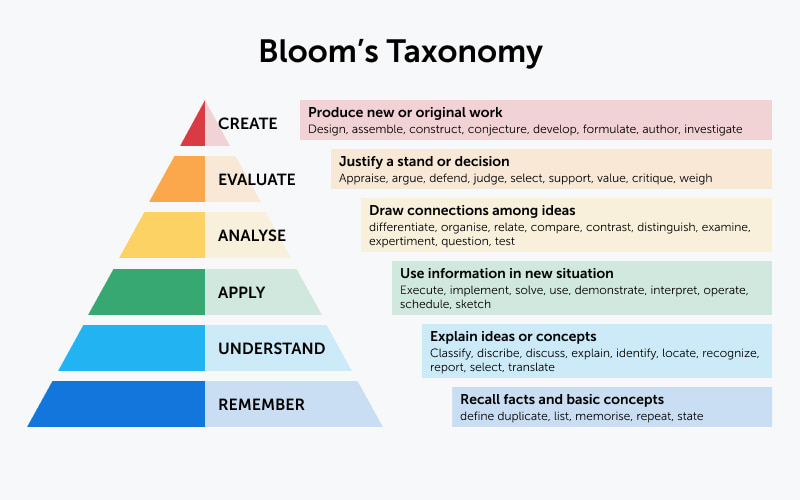
\includegraphics[width=0.75\textwidth]{figures/blooms-taxonomy.jpeg}
    \caption{Hình minh họa Tháp Bloom 6 cấp bậc.}
    \label{fig:blooms_taxonomy}
\end{figure}

Trong ngữ cảnh phân tích ESG, thang Bloom được vận dụng để đánh giá \textbf{mức độ hành động} (actionability) của các phát biểu. Nguyên lý cốt lõi: ngôn ngữ ở mức nhận thức cao phản ánh hành động thực tế cụ thể, trong khi ngôn ngữ ở mức thấp chỉ thể hiện ý định hoặc ghi nhận. Cụ thể, nghiên cứu ánh xạ các động từ theo Bloom sang ba mức hành động:

\begin{itemize}
    \item \textbf{Implemented:} Các động từ ở cấp độ cao ($\geq$ Apply, thì quá khứ) --- ví dụ: \textit{``đã triển khai''}, \textit{``đã giảm 30\% lượng phát thải''}, \textit{``hoàn thành tích hợp hệ thống''}. Đặc biệt, khi đi kèm chỉ số định lượng (KPI), tính cam kết càng mạnh vì tuyên bố trở nên kiểm chứng được~\cite{florstedt2025detecting}.
    \item \textbf{Planning:} Các động từ mang tính định hướng tương lai --- ví dụ: \textit{``sẽ triển khai''}, \textit{``dự kiến đạt mục tiêu vào năm 2030''}, \textit{``lộ trình hướng tới net-zero''}. Các phát biểu này thể hiện ý định nhưng chưa có bằng chứng thực hiện.
    \item \textbf{Indeterminate:} Các phát biểu thiếu tính cam kết cụ thể --- ví dụ: \textit{``nỗ lực hướng tới''}, \textit{``cam kết phát triển bền vững''}, \textit{``góp phần bảo vệ môi trường''}. Đây là nhóm có nguy cơ ESG-washing cao nhất.
\end{itemize}

Bảng ánh xạ chi tiết các mẫu động từ theo Bloom sang nhãn mức độ hành động được trình bày tại Phụ lục~\ref{appendix:grounded_rules}.


\subsection{Hyland Metadiscourse}
\label{subsec:hyland}

Khung Metadiscourse của Hyland~\cite{rodina2007metadiscourse} phân tích cách người viết sử dụng các phương tiện ngôn ngữ để định hướng cách người đọc hiểu và đánh giá nội dung. Trong mô hình này, nhóm Interactional Metadiscourse bao gồm năm phạm trù: hedges, boosters, attitude markers, self-mentions, và engagement markers. Hai phạm trù đặc biệt quan trọng cho phân tích ESG-washing là:

\begin{itemize}
    \item \textbf{Rào đón (Hedging):} Các biểu thức làm giảm mức độ chắc chắn của phát biểu, thể hiện sự né tránh cam kết cụ thể. Ví dụ trong ngữ liệu tiếng Việt: \textit{``nhìn chung''}, \textit{``có thể''}, \textit{``dần dần''}, \textit{``phần nào''}, \textit{``tương đối''}. Rào đón cho phép người viết đưa ra tuyên bố tích cực mà không phải chịu trách nhiệm về tính chính xác --- một chiến lược phổ biến trong ESG-washing.

    \item \textbf{Tăng cường (Boosting):} Các biểu thức nhấn mạnh quá mức, thổi phồng tính chất mà không kèm minh chứng. Ví dụ: \textit{``luôn luôn''}, \textit{``hoàn toàn''}, \textit{``tiên phong''}, \textit{``hàng đầu''}, \textit{``xuất sắc nhất''}. Tăng cường tạo ấn tượng mạnh nhưng không cung cấp thông tin kiểm chứng được.
\end{itemize}

Peng Hu và cộng sự~\cite{su16062571} đã chứng minh rằng các tài liệu có dấu hiệu ESG-washing có xu hướng sử dụng rào đón và tăng cường với tần suất cao hơn đáng kể so với các báo cáo có nội dung ESG thực chất, đồng thời có độ khó đọc (readability) cao hơn --- phản ánh việc sử dụng ngôn ngữ rườm rà để che giấu sự thiếu hụt dữ liệu thực tế.

Ngoài rào đón và tăng cường, nghiên cứu còn hệ thống hóa các mẫu ngôn ngữ \textit{cam kết mơ hồ} (vague commitment) --- các cụm từ mang tính hứa hẹn nhưng thiếu cam kết cụ thể, ví dụ: \textit{``nỗ lực''}, \textit{``đẩy mạnh''}, \textit{``nâng cao nhận thức''}~\cite{florstedt2025detecting}. Tất cả các mẫu này được tổng hợp thành quy tắc ký hiệu để nhận diện các phát biểu \textbf{Indeterminate} (Phụ lục~\ref{appendix:grounded_rules}).


\subsection{Tiêu chuẩn GRI và Mục tiêu Phát triển Bền vững}
\label{subsec:gri}

\subsubsection{Tiêu chuẩn GRI (Global Reporting Initiative)}

GRI là khung tiêu chuẩn lập báo cáo bền vững được sử dụng rộng rãi nhất trên toàn cầu~\cite{gri2021gri}. Bộ tiêu chuẩn GRI 2021 được cấu trúc thành ba nhóm:

\begin{itemize}
    \item \textbf{Tiêu chuẩn phổ quát (Universal Standards --- GRI 1--3):} Quy định nguyên tắc báo cáo, thông tin tổ chức, và phương pháp xác định chủ đề trọng yếu.
    \item \textbf{Tiêu chuẩn theo ngành (Sector Standards):} Hướng dẫn riêng cho từng lĩnh vực kinh tế.
    \item \textbf{Tiêu chuẩn theo chủ đề (Topic Standards):}
    \begin{itemize}
        \item \textit{Nhóm 200 (Kinh tế):} Hiệu quả kinh tế, chống tham nhũng (GRI~205).
        \item \textit{Nhóm 300 (Môi trường):} Nguyên vật liệu (GRI~301), năng lượng (GRI~302), nước (GRI~303), đa dạng sinh học (GRI~304), phát thải (GRI~305), chất thải (GRI~306).
        \item \textit{Nhóm 400 (Xã hội):} Việc làm (GRI~401), quan hệ lao động (GRI~402), an toàn lao động (GRI~403), đào tạo (GRI~404), đa dạng và bình đẳng (GRI~405), cộng đồng (GRI~413), quyền riêng tư khách hàng (GRI~418).
    \end{itemize}
\end{itemize}

Trong nghiên cứu này, các chỉ số GRI được ánh xạ thành hệ thống từ khóa tiếng Việt, phục vụ ba mục đích: (1)~phân loại chủ đề ESG ở mức câu theo các trụ cột E, S, G; (2)~xây dựng quy tắc ký hiệu để kiểm chứng chéo (cross-validation) với nhãn từ mô hình ngôn ngữ; và (3)~cung cấp hệ thống phân cấp chất lượng bằng chứng --- trong đó các bằng chứng tham chiếu đến tiêu chuẩn cụ thể (GRI, ISO, SBTi) được đánh giá cao hơn bằng chứng không có cơ sở quy chuẩn. Bảng ánh xạ chi tiết từ các mã GRI sang từ khóa tiếng Việt được trình bày tại Phụ lục~\ref{appendix:grounded_rules}.


\subsubsection{Mục tiêu Phát triển Bền vững của Liên Hợp Quốc}

Chương trình Nghị sự 2030 của Liên Hợp Quốc gồm 17 Mục tiêu Phát triển Bền vững (SDGs)~\cite{un_sdgs_2015}, cung cấp khung tham chiếu toàn cầu giúp ánh xạ các hoạt động cục bộ của doanh nghiệp vào tiêu chí phổ quát. Các SDG có liên quan trực tiếp đến ngành ngân hàng bao gồm SDG~8 (Việc làm bền vững và tăng trưởng kinh tế), SDG~10 (Giảm bất bình đẳng), SDG~13 (Hành động khí hậu), và SDG~16 (Hòa bình, công lý và thể chế vững mạnh). Trong hệ thống quy tắc ký hiệu, các từ khóa liên quan đến SDG được tích hợp bổ sung cho khung GRI, đặc biệt trong nhóm tài chính toàn diện theo SDG~8 và SDG~10 (Phụ lục~\ref{appendix:grounded_rules}).


%% ============================================================
%% 2.3: XỬ LÝ NGÔN NGỮ TỰ NHIÊN VÀ MÔ HÌNH TRANSFORMER
%% ============================================================
\section{Xử lý ngôn ngữ tự nhiên và mô hình Transformer}
\label{sec:nlp_transformer}

\subsection{Kiến trúc Transformer}
\label{subsec:transformer}

Kiến trúc Transformer, được đề xuất bởi Vaswani và cộng sự~\cite{vaswani2017attention}, là nền tảng của hầu hết các mô hình NLP hiện đại. Khác với các kiến trúc tuần tự trước đó (RNN, LSTM) --- vốn xử lý chuỗi từ trái sang phải hoặc theo hai chiều nhưng với thông tin vị trí bị suy giảm theo khoảng cách --- Transformer xử lý toàn bộ chuỗi đầu vào \textit{song song} nhờ cơ chế self-attention, cho phép mỗi token ``quan sát'' trực tiếp tất cả các token khác trong chuỗi, bất kể khoảng cách.

\begin{figure}[H]
    \centering
    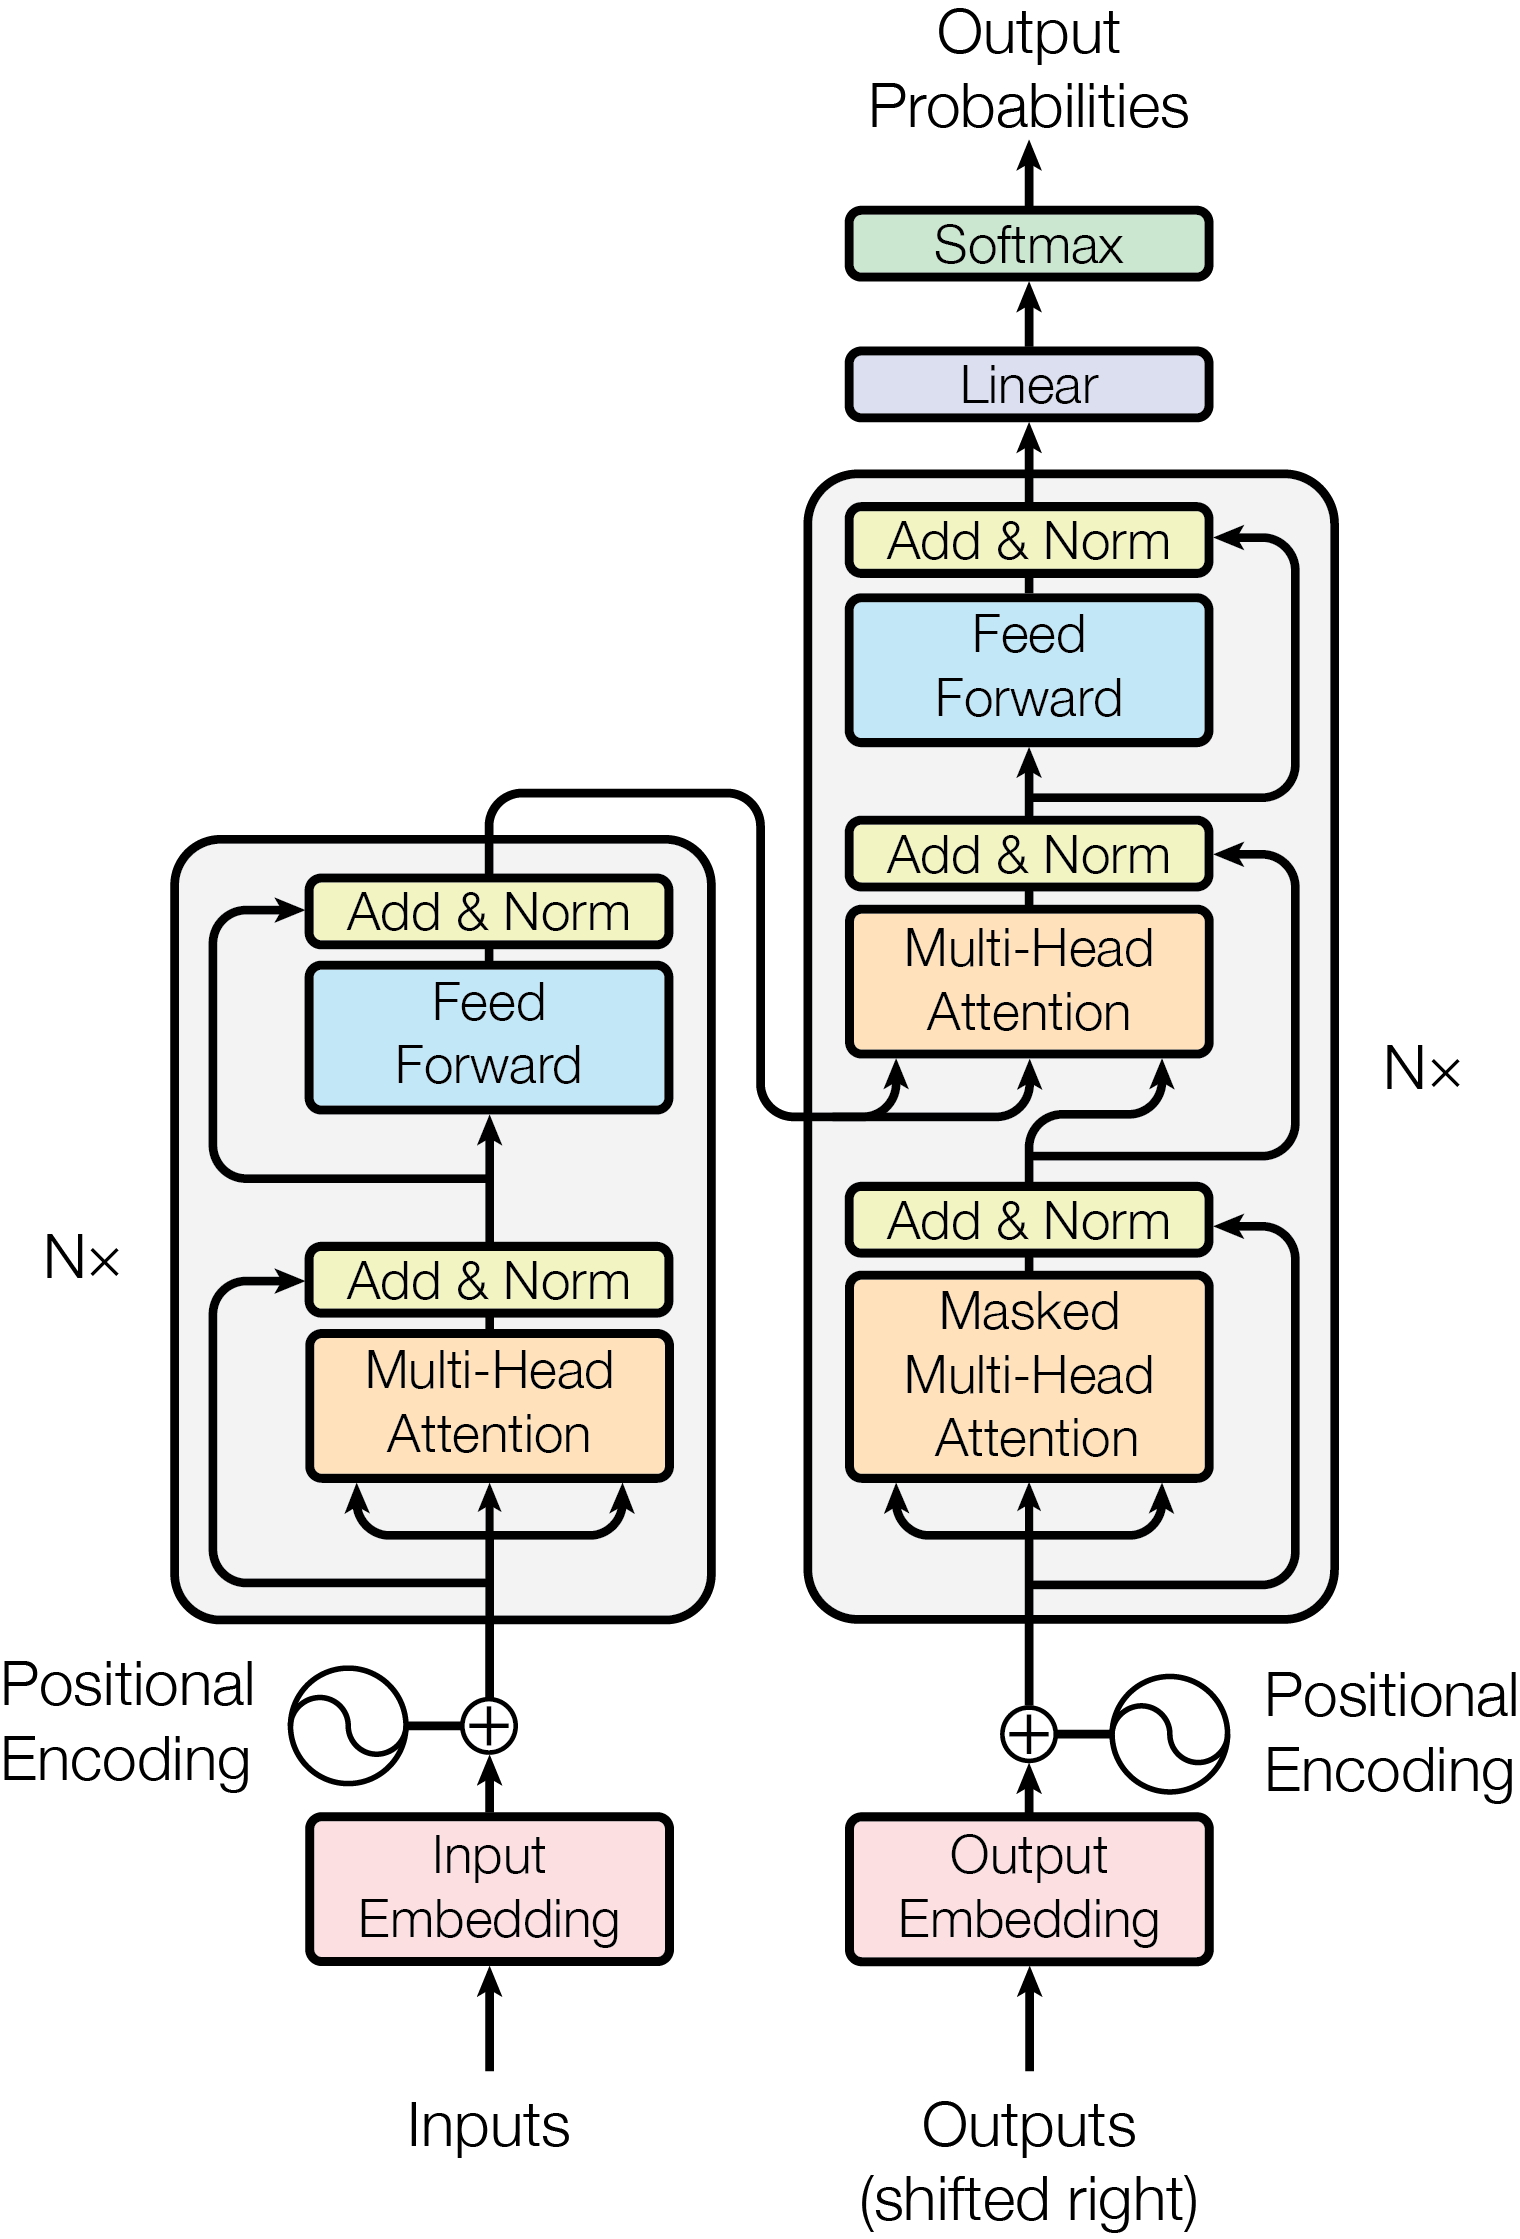
\includegraphics[width=0.55\textwidth]{figures/transformer.png}
    \caption{Kiến trúc Transformer}
    \label{fig:transformer}
\end{figure}

% [TODO: Hình minh họa kiến trúc Transformer — cột Encoder (trái) và Decoder (phải) với các lớp Multi-Head Attention, Feed Forward, Add \& Norm. Xem: Vaswani và cộng sự(2017), Figure 1 "The Transformer — model architecture"]


\subsubsection{Cơ chế Self-attention}

Cho một chuỗi đầu vào $\mathbf{X} = (x_1, x_2, \ldots, x_n)$, cơ chế self-attention tính toán ba ma trận: Query ($\mathbf{Q}$), Key ($\mathbf{K}$), và Value ($\mathbf{V}$) thông qua các phép chiếu tuyến tính:
\begin{equation}
    \mathbf{Q} = \mathbf{X}\mathbf{W}^Q, \quad \mathbf{K} = \mathbf{X}\mathbf{W}^K, \quad \mathbf{V} = \mathbf{X}\mathbf{W}^V
\end{equation}

\noindent trong đó $\mathbf{W}^Q, \mathbf{W}^K \in \mathbb{R}^{d \times d_k}$ và $\mathbf{W}^V \in \mathbb{R}^{d \times d_v}$ là ma trận trọng số học được. Đầu ra của self-attention được tính bằng:
\begin{equation}
    \text{Attention}(\mathbf{Q}, \mathbf{K}, \mathbf{V}) = \text{softmax}\left(\frac{\mathbf{Q}\mathbf{K}^\top}{\sqrt{d_k}}\right)\mathbf{V}
    \label{eq:attention}
\end{equation}

\noindent Hệ số $\frac{1}{\sqrt{d_k}}$ (scaled dot-product) giúp ổn định gradient khi chiều $d_k$ lớn, ngăn giá trị dot-product quá lớn đẩy softmax vào vùng bão hòa.


\subsubsection{Cơ chế Multi-head Attention}

Để nắm bắt nhiều dạng quan hệ ngữ nghĩa khác nhau đồng thời, Transformer sử dụng $h$ đầu chú ý (attention head) song song:
\begin{equation}
    \text{MultiHead}(\mathbf{Q}, \mathbf{K}, \mathbf{V}) = \text{Concat}(\text{head}_1, \ldots, \text{head}_h)\mathbf{W}^O
\end{equation}

\noindent trong đó mỗi $\text{head}_i = \text{Attention}(\mathbf{Q}\mathbf{W}_i^Q, \mathbf{K}\mathbf{W}_i^K, \mathbf{V}\mathbf{W}_i^V)$ là phép attention với bộ trọng số riêng, và $\mathbf{W}^O$ là ma trận chiếu đầu ra. Cơ chế này cho phép mỗi đầu chú ý tập trung vào một khía cạnh quan hệ khác nhau (ví dụ: quan hệ cú pháp, quan hệ ngữ nghĩa, quan hệ tham chiếu).


\subsubsection{Positional Encoding}

Do Transformer xử lý song song không có cấu trúc tuần tự nội tại, thông tin vị trí được bổ sung qua Positional Encoding sử dụng sóng sin:
\begin{align}
    PE_{(pos, 2i)} &= \sin\left(\frac{pos}{10000^{2i/d}}\right) \\
    PE_{(pos, 2i+1)} &= \cos\left(\frac{pos}{10000^{2i/d}}\right)
\end{align}

\noindent trong đó $pos$ là vị trí token trong chuỗi, $i$ là chỉ số chiều, và $d$ là chiều của mô hình. Biểu diễn vị trí được cộng trực tiếp vào embedding đầu vào: $\mathbf{x}'_{pos} = \mathbf{x}_{pos} + PE_{pos}$.

Kiến trúc Transformer hoàn chỉnh gồm Encoder và Decoder, mỗi bộ chứa nhiều lớp xếp chồng với residual connections và layer normalization. Trong các bài toán phân loại văn bản --- bao gồm phân loại ESG --- chỉ phần \textbf{Encoder} được sử dụng, mỗi lớp gồm hai thành phần: Multi-Head Self-Attention và Feed-Forward Network, mỗi thành phần có residual connection và layer normalization.


\subsection{Mô hình ngôn ngữ tiền huấn luyện BERT}
\label{subsec:bert}

BERT được đề xuất bởi Devlin et al.~\cite{devlin2019bert}, là mô hình ngôn ngữ pre-trained dựa trên phần Encoder của Transformer. BERT đánh dấu bước đột phá trong NLP nhờ khả năng học biểu diễn bidirectional --- mỗi token được biểu diễn dựa trên toàn bộ ngữ cảnh xung quanh (cả trái lẫn phải), thay vì chỉ ngữ cảnh một chiều như các mô hình ngôn ngữ hồi quy autoregressive (GPT).

\begin{figure}[H]
    \centering
    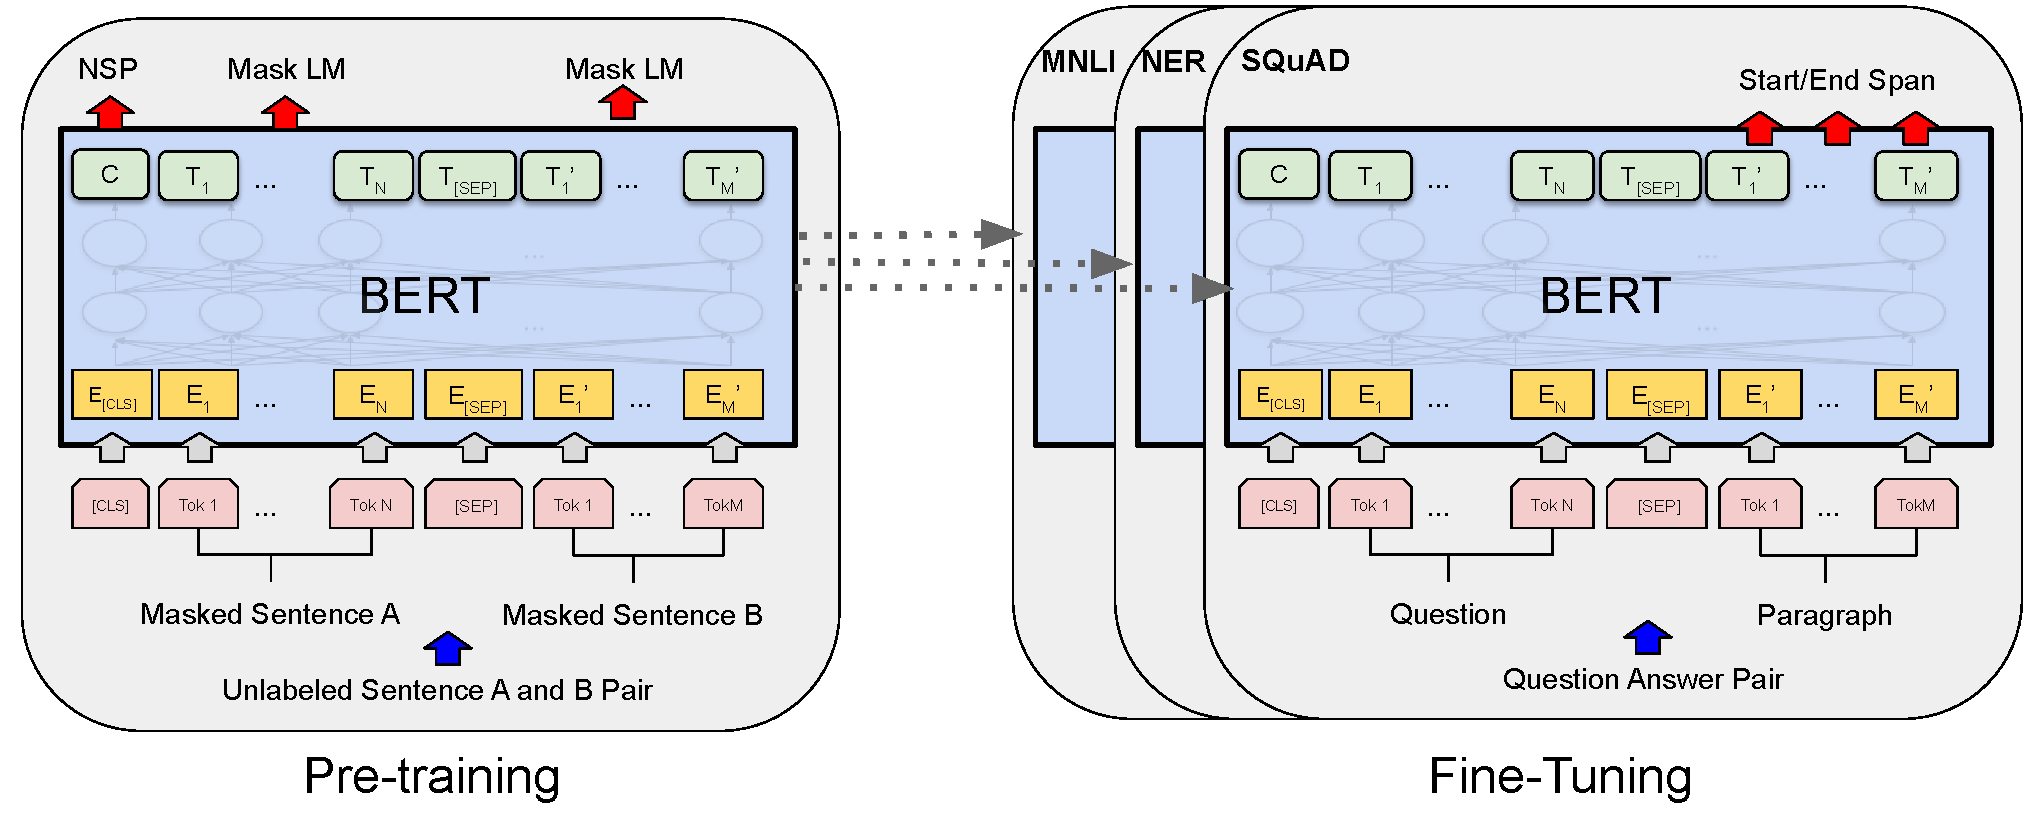
\includegraphics[width=0.75\textwidth]{figures/BERT_Overall.pdf}
    \caption{Kiến trúc BERT — Pre-training (MLM + NSP) và Fine-tuning cho các tác vụ downstream}
    \label{fig:bert}
\end{figure}

% [TODO: Hình minh họa kiến trúc BERT — Pre-training (MLM + NSP) và Fine-tuning cho các tác vụ downstream. Xem: Devlin et al. (2019), Figure 1 "Overall pre-training and fine-tuning procedures for BERT"]

BERT được tiền huấn luyện trên lượng lớn dữ liệu văn bản không gán nhãn với hai nhiệm vụ tự giám sát:

\begin{itemize}
    \item \textbf{Masked Language Modeling (MLM):} Ngẫu nhiên mask 15\% token trong câu đầu vào, mô hình dự đoán các token bị che dựa trên ngữ cảnh hai chiều xung quanh. Nhiệm vụ này buộc mô hình học quan hệ ngữ nghĩa sâu giữa các token, tạo ra biểu diễn phong phú.
    \item \textbf{Next Sentence Prediction (NSP):} Cho cặp câu (A, B), mô hình dự đoán B có phải câu tiếp theo của A trong văn bản gốc hay không. Nhiệm vụ này giúp mô hình nắm bắt quan hệ ngữ nghĩa liên câu.
\end{itemize}

Sau tiền huấn luyện, BERT được tinh chỉnh cho bài toán phân loại bằng cách thêm một lớp phân loại tuyến tính lên biểu diễn token đặc biệt \texttt{[CLS]}:
\begin{equation}
    P(y \mid x) = \text{softmax}(\mathbf{W} \cdot \mathbf{h}_{\texttt{[CLS]}} + \mathbf{b})
    \label{eq:bert_cls}
\end{equation}

\noindent trong đó $\mathbf{h}_{\texttt{[CLS]}} \in \mathbb{R}^d$ là biểu diễn ẩn của token \texttt{[CLS]} ở lớp Transformer cuối cùng, $\mathbf{W} \in \mathbb{R}^{C \times d}$ và $\mathbf{b} \in \mathbb{R}^C$ là trọng số và bias của lớp phân loại ($C$ là số lớp). Toàn bộ mô hình (bao gồm các lớp Transformer đã tiền huấn luyện) được cập nhật trong quá trình fine-tuning với learning rate nhỏ.

Kiến trúc BERT\textsubscript{base} gồm 12 lớp Transformer, 768 chiều ẩn, 12 đầu chú ý ($\sim$110 triệu tham số). BERT\textsubscript{large} gồm 24 lớp, 1024 chiều ẩn, 16 đầu chú ý ($\sim$340 triệu tham số).


\subsection{PhoBERT --- BERT cho tiếng Việt}
\label{subsec:phobert}

PhoBERT~\cite{nguyen2020phobert} là mô hình ngôn ngữ tiền huấn luyện cho tiếng Việt, được phát triển bởi VinAI Research. PhoBERT sử dụng kiến trúc RoBERTa\footnote{RoBERTa (Robustly Optimized BERT Pretraining Approach) là biến thể của BERT với các cải tiến: loại bỏ nhiệm vụ NSP, sử dụng dynamic masking, huấn luyện với batch size lớn hơn và dữ liệu nhiều hơn.} --- một biến thể tối ưu hóa của BERT --- với các đặc điểm:

\begin{itemize}
    \item \textbf{Dữ liệu tiền huấn luyện:} Khoảng 20GB văn bản tiếng Việt từ Wikipedia tiếng Việt và các nguồn tin tức tổng hợp.
    \item \textbf{Tiền xử lý tách từ:} Sử dụng công cụ RDRSegmenter\footnote{RDRSegmenter --- công cụ tách từ tiếng Việt sử dụng mô hình Ripple Down Rules, đạt F1 98\% trên bộ dữ liệu chuẩn VLSP.} để phân đoạn từ tiếng Việt trước khi tokenize. Bước này phản ánh đặc thù ngôn ngữ đơn lập của tiếng Việt, trong đó nhiều từ vựng gồm nhiều âm tiết: \textit{``ngân hàng''} $\rightarrow$ \textit{``ngân\_hàng''}, \textit{``phát triển bền vững''} $\rightarrow$ \textit{``phát\_triển bền\_vững''}.
    \item \textbf{Các phiên bản:}
    \begin{itemize}
        \item \texttt{PhoBERT\textsubscript{base}}: 12 lớp, 768 chiều ẩn, $\sim$135 triệu tham số.
        \item \texttt{PhoBERT\textsubscript{large}}: 24 lớp, 1024 chiều ẩn, $\sim$370 triệu tham số.
    \end{itemize}
\end{itemize}

PhoBERT đạt kết quả vượt trội trên nhiều bài toán NLP tiếng Việt tại thời điểm công bố, bao gồm POS tagging, NER, dependency parsing, và phân loại văn bản~\cite{nguyen2020phobert}. Trong nghiên cứu này, \texttt{PhoBERT\textsubscript{base}} (\texttt{vinai/phobert-base}) được tinh chỉnh cho hai bài toán phân loại nối tiếp: (1)~phân loại chủ đề ESG 6 lớp (E, S\_labor, S\_community, S\_product, G, Non\_ESG) và (2)~phân loại mức độ hành động 3 lớp (Implemented, Planning, Indeterminate).


\subsection{Biểu diễn câu và Sentence Transformers}
\label{subsec:sentence_transformers}

Các mô hình ngôn ngữ như BERT/PhoBERT tạo biểu diễn ở mức token, không được tối ưu cho việc so sánh ngữ nghĩa giữa toàn bộ câu. Reimers và Gurevych~\cite{reimers2019sentence} đề xuất Sentence-BERT (SBERT), sử dụng kiến trúc mạng Siamese/Triplet để tạo biểu diễn câu (sentence embeddings) có ý nghĩa ngữ nghĩa và hiệu quả tính toán.


\subsubsection{Kiến trúc Siamese và phép gộp}

SBERT xử lý hai câu qua cùng một mạng BERT/Transformer chia sẻ trọng số, áp dụng phép gộp (pooling) --- thường là mean pooling (trung bình tất cả token embeddings) --- lên biểu diễn token để thu được vector câu cố định $\mathbf{u}, \mathbf{v} \in \mathbb{R}^d$. Mô hình được huấn luyện trên dữ liệu NLI (cặp câu tương đồng/mâu thuẫn) với hàm mất mát contrastive, sao cho các câu tương đồng ngữ nghĩa có vector gần nhau, các câu khác nghĩa có vector xa nhau. Độ tương đồng ngữ nghĩa giữa hai câu được đo bằng cosine similarity:
\begin{equation}
    \text{sim}(\mathbf{u}, \mathbf{v}) = \frac{\mathbf{u} \cdot \mathbf{v}}{\|\mathbf{u}\| \cdot \|\mathbf{v}\|}
    \label{eq:cosine_sim}
\end{equation}

% [TODO: Hình minh họa kiến trúc Siamese SBERT — hai nhánh BERT chia sẻ trọng số, pooling, cosine similarity. Xem: Reimers & Gurevych (2019), Figure 1]


\subsubsection{Mô hình đa ngôn ngữ}

Trong nghiên cứu này, mô hình \texttt{paraphrase-multilingual-MiniLM-L12-v2} được sử dụng --- một mô hình Sentence Transformer đa ngôn ngữ, được knowledge distillation từ mô hình lớn hơn, hỗ trợ trên 50 ngôn ngữ (bao gồm tiếng Việt), tạo vector câu 384 chiều. Mô hình này được sử dụng trong bước liên kết bằng chứng để tính toán độ tương đồng ngữ nghĩa giữa tuyên bố ESG và các câu bằng chứng tiềm năng trong cùng tài liệu (Chương~3).


%% ============================================================
%% 2.4: SUY LUẬN NGÔN NGỮ TỰ NHIÊN (NLI)
%% ============================================================
\section{Suy luận ngôn ngữ tự nhiên (NLI)}
\label{sec:nli}

\subsection{Bài toán NLI}
\label{subsec:nli_task}

Suy luận ngôn ngữ tự nhiên (Natural Language Inference --- NLI), còn gọi là nhận dạng hàm ý văn bản (Textual Entailment), là bài toán xác định quan hệ logic giữa một cặp câu~\cite{bowman2015large}:

\begin{itemize}
    \item \textbf{Tiền đề (Premise):} Câu cung cấp thông tin nền.
    \item \textbf{Giả thuyết (Hypothesis):} Câu cần kiểm tra tính tương thích logic với tiền đề.
\end{itemize}

\noindent Mô hình NLI phân loại cặp (premise, hypothesis) vào một trong ba quan hệ:

\begin{enumerate}
    \item \textbf{Hàm ý (Entailment):} Giả thuyết được suy ra một cách logic từ tiền đề. Ví dụ: Premise = ``Ngân hàng đã giảm 30\% lượng CO$_2$'', Hypothesis = ``Ngân hàng thực hiện giảm phát thải'' $\rightarrow$ Entailment.
    \item \textbf{Trung lập (Neutral):} Giả thuyết không mâu thuẫn nhưng cũng không được suy ra trực tiếp từ tiền đề.
    \item \textbf{Mâu thuẫn (Contradiction):} Giả thuyết mâu thuẫn với nội dung tiền đề. Ví dụ: Premise = ``Tổng phát thải tăng 15\% so với năm trước'', Hypothesis = ``Ngân hàng cam kết giảm phát thải hàng năm'' $\rightarrow$ Contradiction.
\end{enumerate}

Bộ dữ liệu SNLI (Stanford Natural Language Inference)~\cite{bowman2015large} gồm khoảng 570.000 cặp câu tiếng Anh được gán nhãn thủ công, là bộ dữ liệu chuẩn mực (benchmark) cho bài toán NLI. Conneau et al.~\cite{conneau2018xnli} mở rộng sang XNLI (Cross-lingual Natural Language Inference) với 15 ngôn ngữ, cho phép đánh giá khả năng suy luận đa ngôn ngữ của các mô hình, bao gồm cả zero-shot transfer từ tiếng Anh sang các ngôn ngữ khác.

\textbf{Ứng dụng trong phân tích ESG.} Trong nghiên cứu này, NLI được vận dụng như cơ chế xác minh quan hệ logic giữa tuyên bố ESG và bằng chứng được truy xuất. Đây là bước thứ hai trong pipeline liên kết bằng chứng hai giai đoạn (Chương~3):
\begin{itemize}
    \item \textit{Entailment:} Bằng chứng hỗ trợ trực tiếp cho tuyên bố $\rightarrow$ tăng điểm bằng chứng (Evidence Strength), giảm rủi ro ESG-washing.
    \item \textit{Neutral:} Bằng chứng liên quan về mặt chủ đề nhưng không xác nhận $\rightarrow$ không thay đổi đánh giá.
    \item \textit{Contradiction:} Bằng chứng mâu thuẫn với tuyên bố $\rightarrow$ khuếch đại rủi ro ESG-washing (hệ số nhân 1,3$\times$).
\end{itemize}


\subsection{NLI đa ngôn ngữ và mô hình DeBERTa}
\label{subsec:deberta}

\subsubsection{Kiến trúc DeBERTa}

DeBERTa (Decoding-enhanced BERT with Disentangled Attention)~\cite{he2021deberta} cải tiến BERT qua hai cơ chế chính:

\begin{itemize}
    \item \textbf{Disentangled Attention:} Thay vì gộp thông tin nội dung và vị trí thành một vector duy nhất rồi tính attention (như BERT), DeBERTa biểu diễn chúng bằng hai vector riêng biệt. Ma trận attention được tính từ tổ hợp ba thành phần:
    \begin{itemize}
        \item \textit{Content-to-Content:} Quan hệ ngữ nghĩa giữa các token (``ngân\_hàng'' liên quan ``tín\_dụng'').
        \item \textit{Content-to-Position:} Ảnh hưởng của nội dung lên vị trí tương đối (động từ chính thường ở vị trí cố định so với chủ ngữ).
        \item \textit{Position-to-Content:} Ảnh hưởng của vị trí tương đối lên cách hiểu nội dung (token đầu câu thường mang trọng số chủ đề cao hơn).
    \end{itemize}

    \item \textbf{Enhanced Mask Decoder:} Bổ sung absolute position vào lớp giải mã cuối cùng, kết hợp với relative position đã được sử dụng trong các lớp attention trước đó. Sự kết hợp này giúp mô hình phân biệt chính xác hơn các từ đồng âm khác nghĩa phụ thuộc vị trí.
\end{itemize}


\subsubsection{mDeBERTa-v3 cho NLI đa ngôn ngữ}

Mô hình \texttt{mDeBERTa-v3-base-xnli-multilingual-nli-2mil7}~\cite{laurer2023building} là phiên bản DeBERTa đa ngôn ngữ được tinh chỉnh trên hơn 2,7 triệu cặp câu NLI từ nhiều bộ dữ liệu (SNLI, MultiNLI, ANLI, FEVER-NLI, LingNLI), hỗ trợ hơn 100 ngôn ngữ bao gồm tiếng Việt. Laurer et al.~\cite{laurer2023building} chứng minh rằng các mô hình NLI đa ngôn ngữ --- khi được huấn luyện trên đủ dữ liệu --- có thể đạt hiệu quả zero-shot classification cạnh tranh với các mô hình được tinh chỉnh riêng cho từng ngôn ngữ.

Trong nghiên cứu này, mô hình mDeBERTa-v3 được sử dụng trong bước xác minh NLI của pipeline liên kết bằng chứng, với nhiệm vụ phân loại cặp (tuyên bố ESG, bằng chứng truy xuất) thành ba nhãn \{Entailment, Neutral, Contradiction\}, ngưỡng entailment $\geq 0{,}5$.


%% ============================================================
%% 2.5: TRÍ TUỆ NHÂN TẠO LAI GHÉP NEURO-SYMBOLIC
%% ============================================================
\section{Trí tuệ nhân tạo lai ghép Neuro-Symbolic}
\label{sec:neuro_symbolic}

\subsection{Khái niệm và phân loại theo Kautz}
\label{subsec:neuro_symbolic_overview}

AI lai ghép Neuro-Symbolic là hướng tiếp cận kết hợp hai nhánh truyền thống của AI~\cite{kautz2022third}:

\begin{itemize}
    \item \textbf{Hệ kết nối (Neural/Connectionist):} Các mô hình dựa trên mạng nơ-ron (deep learning), có khả năng học biểu diễn từ dữ liệu, xử lý ngôn ngữ tự nhiên linh hoạt, nhưng hoạt động như ``hộp đen'' --- thiếu tính giải thích (explainability) và dễ tạo ra ảo giác (hallucination).
    \item \textbf{Hệ ký hiệu (Symbolic):} Hệ thống dựa trên quy tắc logic hình thức, có tính giải thích cao và đảm bảo tính nhất quán logic, nhưng thiếu linh hoạt, khó mở rộng cho ngôn ngữ tự nhiên, và có recall thấp do phụ thuộc vào độ phủ của luật.
\end{itemize}

Kautz~\cite{kautz2022third} đề xuất phân loại AI Neuro-Symbolic thành sáu cấp (Type 1--6) dựa trên mức độ tích hợp giữa hai thành phần, từ kết hợp lỏng lẻo đến tích hợp sâu:

\begin{table}[htbp]
\centering
\caption{Phân loại AI Neuro-Symbolic theo Kautz~\cite{kautz2022third}}
\label{tab:kautz_taxonomy}
\small
\renewcommand{\arraystretch}{1.2}
\begin{tabular}{|c|l|p{8cm}|}
\hline
\textbf{Type} & \textbf{Ký hiệu} & \textbf{Mô tả} \\
\hline
1 & Symbolic $\rightarrow$ Neural & Hệ ký hiệu sử dụng neural network như thành phần con \\
\hline
2 & Neural $|$ Symbolic & Hai hệ thống chạy song song, kết quả tổng hợp \\
\hline
3 & Neural $\rightarrow$ Symbolic & Neural giải quyết bài toán, kết quả diễn giải bằng logic \\
\hline
4 & Neural[Symbolic] & Tri thức ký hiệu biên dịch vào kiến trúc hoặc hàm mất mát neural \\
\hline
5 & Neural $\leftrightarrow$ Symbolic & Tích hợp sâu hai chiều --- ký hiệu ảnh hưởng neural và ngược lại \\
\hline
6 & Neural = Symbolic & Tích hợp hoàn toàn --- không phân biệt hai thành phần \\
\hline
\end{tabular}
\end{table}

Nghiên cứu này vận dụng sự kết hợp giữa \textbf{Type~4} và \textbf{Type~5}: tri thức ký hiệu từ các khung GRI, Bloom, và Hyland (Mục~\ref{sec:linguistic_frameworks}) được biên dịch thành các ràng buộc mệnh đề logic, tích hợp vào hàm mất mát ngữ nghĩa trong quá trình huấn luyện mô hình PhoBERT (Type~4), đồng thời điều chỉnh dự đoán qua suy luận có ràng buộc tại thời điểm inference (Type~5).


\subsection{Hàm mất mát ngữ nghĩa}
\label{subsec:semantic_loss}

Xu et al.~\cite{xu2018semantic} đề xuất hàm mất mát ngữ nghĩa (semantic loss function) tại hội nghị ICML 2018 --- một cơ chế tích hợp tri thức ký hiệu dạng mệnh đề logic vào quá trình huấn luyện mạng nơ-ron thông qua hàm mất mát. Ý tưởng cốt lõi: thay vì dùng quy tắc logic để lọc nhãn trước khi huấn luyện (hard constraint), semantic loss ``mềm hóa'' ràng buộc thành một thành phần \textit{khả vi} (differentiable) trong hàm mất mát, cho phép gradient descent \textit{vừa} học từ dữ liệu \textit{vừa} tuân thủ tri thức miền.


\subsubsection{Ý tưởng hình thức}

Cho ràng buộc logic $\alpha$ (ví dụ: ``mỗi câu chỉ thuộc đúng một lớp'') và vector xác suất đầu ra $\mathbf{p} = (p_1, p_2, \ldots, p_C)$ từ softmax của mô hình, semantic loss đo lường \textit{xác suất mà đầu ra vi phạm $\alpha$}:
\begin{equation}
    L_{\text{semantic}}(\alpha, \mathbf{p}) = -\log P(\alpha \mid \mathbf{p}) = -\log \sum_{\mathbf{y} \models \alpha} \prod_{i} p_i^{y_i}(1-p_i)^{1-y_i}
    \label{eq:semantic_loss_general}
\end{equation}

\noindent trong đó tổng lấy trên tất cả các phép gán nhị phân $\mathbf{y} \in \{0,1\}^C$ thỏa mãn ràng buộc $\alpha$, và $y_i$ cho biết lớp $i$ có được chọn hay không. Trực giác: khi tất cả phép gán thỏa mãn đều có xác suất cao, $L_{\text{semantic}} \rightarrow 0$; khi các phép gán vi phạm có xác suất cao, $L_{\text{semantic}} \rightarrow +\infty$.


\subsubsection{Các ràng buộc cụ thể trong nghiên cứu}

Nghiên cứu biên dịch tri thức miền thành ba dạng ràng buộc mệnh đề logic:

\textbf{(1) Ràng buộc Exactly-One.} Đảm bảo mỗi câu thuộc \textit{đúng} một lớp --- tương đương phép toán XOR trên $C$ biến Boolean:
\begin{equation}
    \alpha_1: \bigoplus_{i=1}^{C} X_i \equiv \left(\bigvee_{i=1}^{C} X_i\right) \wedge \bigwedge_{i < j} \left(\neg X_i \vee \neg X_j\right)
\end{equation}

Semantic loss cho ràng buộc này:
\begin{equation}
    L_{\text{exactly\_one}}(\mathbf{p}) = -\log\left(\sum_{i=1}^{C} p_i \prod_{j \neq i}(1 - p_j)\right)
    \label{eq:exactly_one}
\end{equation}

\noindent Giá trị bằng 0 khi đúng một $p_i = 1$ và các $p_j = 0$ ($j \neq i$), phạt nặng khi phân bố xác suất không rõ ràng. Xu et al.~\cite{xu2018semantic} chỉ ra công thức có thể được tính toán hiệu quả dưới dạng $\prod_j(1-p_j) \times \sum_i \frac{p_i}{1-p_i}$, tránh chi phí tính toán mũ theo số lớp.

\textbf{(2) Ràng buộc Implication (Hàm ý).} Khi quy tắc ký hiệu phát hiện bằng chứng textual cho nhãn $k$ với mức độ tin cậy $t \in [0,1]$ (fuzzy truth value từ fuzzy evaluation), ràng buộc hàm ý được mã hóa thành:
\begin{equation}
    L_{\text{impl}}(t, p_k) = -t \cdot \log(p_k)
    \label{eq:implication}
\end{equation}

\noindent Ràng buộc này ``kéo'' xác suất $p_k$ lên cao khi quy tắc ký hiệu kích hoạt mạnh. Ví dụ: nếu quy tắc GRI~302 (Energy) phát hiện từ khóa \textit{``năng lượng tái tạo''} với $t = 0{,}8$, loss sẽ phạt mô hình nếu $p_{\text{E}}$ thấp.

\textbf{(3) Ràng buộc Negation (Phủ định).} Khi bằng chứng ký hiệu chỉ ra câu \textit{không nên} thuộc lớp $k$ --- ví dụ: phát hiện Hedging (Hyland) $\rightarrow$ không phải Implemented:
\begin{equation}
    L_{\text{neg}}(t, p_k) = -t \cdot \log(1 - p_k)
    \label{eq:negation}
\end{equation}


\subsubsection{Hàm mất mát tổng}

Hàm mất mát tổng kết hợp cross-entropy truyền thống (học từ dữ liệu gán nhãn) với semantic loss (tuân thủ tri thức miền):
\begin{equation}
    L_{\text{total}} = L_{\text{CE}} + \lambda \cdot \Big(w_1 \cdot L_{\text{exactly\_one}} + w_2 \cdot \overline{L}_{\text{impl}} + w_3 \cdot \overline{L}_{\text{neg}}\Big)
    \label{eq:total_loss}
\end{equation}

\noindent trong đó $\lambda$ là trọng số tổng thể của thành phần semantic loss, $w_1, w_2, w_3$ là trọng số từng loại ràng buộc, và $\overline{L}_{\text{impl}}, \overline{L}_{\text{neg}}$ là giá trị trung bình trên các ràng buộc kích hoạt trong batch.

Kiến trúc này mang lại sự \textit{cân bằng giữa tính linh hoạt và tính nhất quán logic}: $L_{\text{CE}}$ cho phép mô hình PhoBERT học các mẫu phức tạp từ dữ liệu huấn luyện, trong khi $L_{\text{semantic}}$ đảm bảo các dự đoán tuân thủ tri thức miền đã được hệ thống hóa từ GRI, Bloom Taxonomy, và Hyland Metadiscourse.


\subsection{Suy luận có ràng buộc tại thời điểm dự đoán}
\label{subsec:constrained_inference}

Ngoài việc tích hợp tri thức ký hiệu trong huấn luyện qua semantic loss, nghiên cứu cũng áp dụng phương pháp suy luận hậu nghiệm có ràng buộc (posterior regularization) tại thời điểm dự đoán (inference). Phân phối xác suất cuối cùng được tính theo mô hình \textit{log-linear} (product-of-experts):
\begin{equation}
    \log P(y \mid x) = (1 - \alpha) \cdot \log P_{\text{neural}}(y \mid x) + \alpha \cdot \log P_{\text{rules}}(y \mid x)
    \label{eq:constrained_inference}
\end{equation}

\noindent trong đó:
\begin{itemize}
    \item $P_{\text{neural}}(y \mid x)$ là phân phối softmax từ mô hình PhoBERT.
    \item $P_{\text{rules}}(y \mid x)$ là phân phối từ hệ quy tắc ký hiệu, được tính từ tổng hợp các bằng chứng implication và negation qua softmax:
    \begin{equation}
        P_{\text{rules}}(k \mid x) \propto \exp\left(\sum_r t_r^{(k)} - \sum_r t_r^{(\neg k)}\right)
    \end{equation}
    trong đó $t_r^{(k)}$ là truth value của quy tắc hàm ý cho lớp $k$, và $t_r^{(\neg k)}$ là truth value của quy tắc phủ định lớp $k$.
    \item $\alpha \in [0,1]$ là trọng số trộn, được tối ưu bằng grid search trên tập validation.
\end{itemize}

Phương pháp này cho phép hệ thống cung cấp kết quả \textit{có tính giải thích} (explainable): mỗi dự đoán không chỉ đưa ra nhãn mà còn đi kèm danh sách các quy tắc kích hoạt, mức độ ảnh hưởng, và chỉ báo liệu dự đoán cuối cùng khác biệt so với dự đoán thuần neural (rule-adjusted).


%% ============================================================
%% 2.6: CHẮT LỌC TRI THỨC
%% ============================================================
\section{Chắt lọc tri thức}
\label{sec:knowledge_distillation}

Chắt lọc tri thức (Knowledge Distillation), được hình thức hóa bởi Hinton et al.~\cite{hinton2015distilling}, là phương pháp truyền tri thức từ một teacher model (mô hình lớn, phức tạp) sang một student model (mô hình nhỏ hơn, hiệu quả hơn) mà vẫn giữ được phần lớn hiệu năng.

Ý tưởng cốt lõi: thay vì chỉ học từ hard labels $y \in \{0, 1\}$, student học từ \textit{soft targets} $\mathbf{q}$ của teacher --- phân phối xác suất mềm chứa thông tin phong phú hơn về quan hệ giữa các lớp (``dark knowledge''). Ví dụ, trong bài toán phân loại ESG, khi teacher dự đoán một câu là E (Môi trường) với xác suất 0{,}85, đồng thời gán S (Xã hội) xác suất 0{,}10 --- thông tin rằng ``câu này chủ yếu về E nhưng có liên quan nhẹ đến S'' là tri thức mà hard label đơn thuần không truyền tải được.

Hàm mất mát của chắt lọc tri thức kết hợp hai thành phần:
\begin{equation}
    L_{\text{KD}} = (1 - \beta) \cdot L_{\text{CE}}(y, \hat{y}) + \beta \cdot \tau^2 \cdot D_{\text{KL}}(\mathbf{q}_\tau \| \hat{\mathbf{p}}_\tau)
    \label{eq:kd_loss}
\end{equation}

\noindent trong đó:
\begin{itemize}
    \item $L_{\text{CE}}(y, \hat{y})$: Cross-entropy với nhãn cứng --- đảm bảo student vẫn học đúng lớp.
    \item $D_{\text{KL}}(\mathbf{q}_\tau \| \hat{\mathbf{p}}_\tau)$: Divergence Kullback--Leibler giữa soft targets và dự đoán student.
    \item $\mathbf{q}_\tau = \text{softmax}(\mathbf{z}_{\text{teacher}} / \tau)$: Phân phối teacher được ``làm phẳng'' bằng temperature $\tau > 1$.
    \item $\beta$: Trọng số cân bằng giữa hai thành phần.
    \item $\tau^2$: Hệ số bù gradient bị thu nhỏ khi $\tau$ tăng.
\end{itemize}

Trong paradigm hiện đại, các mô hình ngôn ngữ lớn (LLM) có thể đóng vai trò teacher model để tạo nhãn tự động (silver labels) cho dữ liệu không gán nhãn, thay thế quá trình gán nhãn thủ công tốn kém. Quy trình này đặc biệt phù hợp khi:

\begin{itemize}
    \item Dữ liệu gán nhãn thủ công không khả thi hoặc quá tốn kém --- ví dụ: phân loại ESG cho hàng chục nghìn câu tiếng Việt đòi hỏi chuyên gia có kiến thức cả về tài chính lẫn ngôn ngữ.
    \item Mô hình student cần chạy hiệu quả trong production --- LLM quá lớn và tốn tài nguyên để triển khai trực tiếp trên toàn bộ pipeline.
    \item Có sẵn tri thức miền (domain knowledge) có thể được mã hóa vào prompt của LLM để hướng dẫn quá trình gán nhãn, tận dụng khả năng in-context learning.
\end{itemize}

Tuy nhiên, nhãn từ LLM (silver labels) không hoàn hảo --- chúng có thể chứa nhiễu do hallucination, thiếu nhất quán, hoặc thiếu ngữ cảnh miền chuyên sâu. Do đó, quy trình chắt lọc tri thức trong nghiên cứu này bổ sung một bước quan trọng: \textit{đối chiếu nhãn LLM với quy tắc ký hiệu} (từ GRI, Bloom, Hyland) để nâng cao chất lượng nhãn --- nhãn được cả LLM lẫn quy tắc đồng thuận sẽ có độ tin cậy cao hơn nhãn chỉ từ một nguồn. Chi tiết quy trình được trình bày tại Chương~3.


%% ============================================================
%% 2.7: CÁC NGHIÊN CỨU LIÊN QUAN
%% ============================================================
\section{Các nghiên cứu liên quan}
\label{sec:related_works}

Lĩnh vực phát hiện ESG-washing bằng phương pháp tính toán đã phát triển nhanh chóng từ năm 2023, với nhiều hướng tiếp cận khác nhau. Phần này tổng hợp và phân tích các nghiên cứu tiêu biểu, đồng thời chỉ ra khoảng trống mà nghiên cứu này nhằm lấp đầy.


\subsection{Phát hiện ESG-washing bằng phân tích ngôn ngữ}
\label{subsec:rw_linguistic}

Florstedt và Fahlbusch~\cite{florstedt2025detecting} đề xuất một khung NLP kết hợp để phát hiện các phát ngôn mang tính ``cheap talk'' trong báo cáo về phát thải khí nhà kính. Phương pháp sử dụng VADER cho phân tích cảm xúc, ClimateBERT cho đánh giá độ cụ thể ngôn ngữ, và Sentence-BERT cho truy xuất bằng chứng nội tại. Kết quả thực nghiệm cho thấy các phát biểu tích cực nhưng thiếu tính cụ thể, đặc biệt khi không có bằng chứng hỗ trợ nội tại, thường gắn với nguy cơ ESG-washing cao. Tuy nhiên, khung mô hình chủ yếu áp dụng cho tiếng Anh, chưa xử lý hiệu quả các câu ghép, và chưa tích hợp cơ chế suy luận logic để kiểm định bằng chứng một cách hệ thống.

Hu et al.~\cite{su16062571} phân tích ESG-washing qua góc độ \textit{độ khó đọc} (readability) của báo cáo. Nghiên cứu chứng minh rằng doanh nghiệp có hành vi ESG-washing có xu hướng viết báo cáo rườm rà, lạm dụng cấu trúc phức tạp nhằm che giấu việc thiếu thông tin định lượng, tạo ra ``cheap talk'' bảo vệ hình ảnh.

Zhao et al.~\cite{zhao2023detecting} áp dụng NLP để phát hiện greenwashing trên ba trụ cột ESG, mở đường cho việc sử dụng kiến trúc Transformer thay cho TF-IDF truyền thống trong phân tích tài chính bền vững.


\subsection{Phát hiện từ đối chiếu nguồn dữ liệu bên ngoài}
\label{subsec:rw_external}

Lipenkova et al.~\cite{lipenkova2023detecting} so sánh nội dung ESG trong báo cáo doanh nghiệp Đức với thông tin từ báo chí và tổ chức phi chính phủ. Sử dụng sentence embeddings và mô hình Transformer, nhóm nghiên cứu phát hiện rằng các công ty tự đánh giá ESG quá tích cực trong khi bên thứ ba phản ánh trái ngược thường có nguy cơ ESG-washing cao. Tuy nhiên, cách tiếp cận này phụ thuộc vào sự sẵn có của nguồn dữ liệu bên ngoài đáng tin cậy --- điều không khả thi ở nhiều thị trường mới nổi như Việt Nam, nơi báo chí ESG và dữ liệu giám sát độc lập còn hạn chế.

Kathan et al.~\cite{kathan2025you} so sánh điểm ESG từ các tổ chức xếp hạng (MSCI, Sustainalytics) với các tín hiệu greenwashing thực tế, chỉ ra rằng điểm ESG cao không đồng nghĩa với rủi ro tẩy xanh thấp --- một phát hiện ủng hộ nhu cầu phân tích trực tiếp nội dung tài liệu thay vì phụ thuộc vào điểm xếp hạng.

Lagasio~\cite{lagasio2024esg} đề xuất chỉ số định lượng ESG-washing Severity Index (ESGSI) dựa trên TF-IDF, LDA và phân tích cảm xúc, đo lường sự lệch giữa ngôn ngữ tích cực và nội dung ESG thực chất. Ứng dụng trên 749 doanh nghiệp, ESGSI cho thấy sự chênh lệch rõ rệt giữa các ngành và khu vực. Tuy nhiên, ESGSI chỉ phản ánh độ lệch tương đối về hình thức, không đánh giá tính nhất quán logic hay tính kiểm chứng thực tế của nội dung.


\subsection{Tổng hợp và khoảng trống nghiên cứu}
\label{subsec:rw_gap}

Bảng~\ref{tab:related_work_comparison} tổng hợp so sánh các nghiên cứu liên quan theo năm tiêu chí: phương pháp chính, phân tích ở mức câu, hỗ trợ đa ngôn ngữ, chỉ sử dụng dữ liệu nội tại (không phụ thuộc nguồn ngoài), và tích hợp suy luận logic.

\begin{table}[htbp]
\centering
\caption{So sánh các nghiên cứu liên quan về phát hiện ESG-washing}
\label{tab:related_work_comparison}
\small
\renewcommand{\arraystretch}{1.3}
\begin{tabular}{|p{3cm}|p{2.8cm}|c|c|c|c|}
\hline
\textbf{Nghiên cứu} & \textbf{Phương pháp} & \textbf{Mức câu} & \textbf{Đa NN} & \textbf{Nội tại} & \textbf{Logic} \\
\hline
Florstedt et al. \cite{florstedt2025detecting} & VADER + SBERT & \checkmark & & \checkmark & \\
\hline
Lipenkova et al. \cite{lipenkova2023detecting} & Sentence Emb. & & & & \\
\hline
Lagasio \cite{lagasio2024esg} & TF-IDF + LDA & & & \checkmark & \\
\hline
Zhao et al. \cite{zhao2023detecting} & Transformer & \checkmark & & \checkmark & \\
\hline
Kathan et al. \cite{kathan2025you} & ESG scores & & & & \\
\hline
Hu et al. \cite{su16062571} & Readability & & & \checkmark & \\
\hline
\textbf{Nghiên cứu này} & \textbf{Neuro-Symbolic} & \checkmark & \checkmark & \checkmark & \checkmark \\
\hline
\end{tabular}
\end{table}

Từ phân tích trên, ba khoảng trống chính được xác định:

\begin{enumerate}
    \item \textbf{Thiếu phân tích ở mức câu kết hợp suy luận logic.} Đa số nghiên cứu chỉ phân tích ở mức tài liệu hoặc sử dụng chỉ số tổng hợp, thiếu khả năng truy vết (traceability) đến từng tuyên bố cụ thể. Các nghiên cứu có phân tích mức câu~\cite{florstedt2025detecting, zhao2023detecting} chưa tích hợp cơ chế suy luận logic để kiểm định tính nhất quán giữa tuyên bố và bằng chứng.

    \item \textbf{Phụ thuộc dữ liệu bên ngoài.} Nhiều phương pháp~\cite{lipenkova2023detecting, kathan2025you} đòi hỏi dữ liệu ESG từ bên thứ ba (điểm xếp hạng, tin tức), không khả thi tại các thị trường mới nổi thiếu hạ tầng giám sát ESG độc lập.

    \item \textbf{Chưa hỗ trợ ngôn ngữ tiếng Việt.} Tất cả các nghiên cứu hiện có đều tập trung vào tiếng Anh hoặc tiếng Đức, chưa có công trình phát hiện ESG-washing trực tiếp trên văn bản tiếng Việt --- một ngôn ngữ đơn lập với đặc thù hình thái và ngữ nghĩa riêng.
\end{enumerate}

Nghiên cứu này nhằm lấp đầy các khoảng trống trên bằng cách: (1)~phân tích ESG-washing ở mức câu với phương pháp neuro-symbolic tích hợp tri thức miền từ GRI, Bloom, và Hyland; (2)~chỉ sử dụng dữ liệu nội tại trong cùng tài liệu (intra-document evidence linking); và (3)~áp dụng trực tiếp cho ngữ liệu tiếng Việt thông qua mô hình PhoBERT~\cite{nguyen2020phobert} kết hợp NLI đa ngôn ngữ~\cite{laurer2023building}.
